% -----------------------------*- LaTeX -*------------------------------
\documentclass[UTF8]{report}
% ------------------------------------------------------------------------
% Packages
% ------------------------------------------------------------------------
\usepackage{ctex}
\usepackage[body={7in, 9in},left=1in,right=1in]{geometry}
\usepackage{amsmath,amsfonts,amssymb,bm,amsthm}%数学宏包、数学字体、数学符号、支持 \mathscr{} 字体、支持粗斜体 \bm{}、数学定理
\usepackage{graphicx}%支持 \includegraphics{} 插图
\usepackage{subfigure}%插入子图
\usepackage{nicefrac}
\usepackage{mathrsfs}
\usepackage{caption}
\usepackage{algorithm,algorithmicx}
\usepackage[noend]{algpseudocode}
\usepackage{fancyhdr}
\usepackage{adjustbox}
\usepackage{esint}%支持多种积分算子
\usepackage{mathtools}%数学宏包的重要补充
\usepackage{upgreek}%数学环境的直立希腊字母
\usepackage{enumitem}%自定义列表环境
\usepackage{color}%支持颜色改变
\usepackage{extarrows}%任意长度的箭头
\usepackage{tikz,xcolor}%画图、画 F eynman 图
\usepackage{breqn}
\usepackage{fontsize}
\usepackage[framemethod=TikZ]{mdframed}
\usepackage{fontspec}
\usepackage{bigstrut,multirow,rotating}%Excel表格自动导入latex
\usepackage{booktabs}
\usepackage{scribe}
% ------------------------------------------------------------------------
% Macros
% ------------------------------------------------------------------------
%~~~~~~~~~~~~~~~
% Utility latin
%~~~~~~~~~~~~~~~
\newcommand{\ie}{\textit{i.e.}}
\newcommand{\eg}{\textit{e.g.}}
%~~~~~~~~~~~~~~~
% Environment shortcuts
%~~~~~~~~~~~~~~~
\newcommand{\balign}[1]{\ealign{\begin{align}#1\end{align}}}
\newcommand{\baligns}[1]{\ealigns{\begin{align*}#1\end{align*}}}
\newcommand{\bitemize}[1]{\eitemize{\begin{itemize}#1\end{itemize}}}
\newcommand{\benumerate}[1]{\eenumerate{\begin{enumerate}#1\end{enumerate}}}
%~~~~~~~~~~~~~~~
% Text with quads around it
%~~~~~~~~~~~~~~~
\newcommand{\qtext}[1]{\quad\text{#1}\quad}
%~~~~~~~~~~~~~~~
% Shorthand for math formatting
%~~~~~~~~~~~~~~~
\newcommand{\mbb}[1]{\mathbb{#1}}
\newcommand{\mbi}[1]{\boldsymbol{#1}} % Bold and italic (math bold italic)
\newcommand{\mbf}[1]{\mathbf{#1}}
\newcommand{\mc}[1]{\mathcal{#1}}
\newcommand{\mrm}[1]{\mathrm{#1}}
\newcommand{\tbf}[1]{\textbf{#1}}
\newcommand{\tsc}[1]{\textsc{#1}}
%\def\<{{\langle}}
%\def\>{{\rangle}}
\newcommand{\sT}{\sf T}
\newcommand{\grad}{\nabla}
\newcommand{\Proj}{\Pi}
%~~~~~~~~~~~~~~~
% Common sets 定义数集符号
%~~~~~~~~~~~~~~~
\newcommand{\R}{\mathbb{R}}
\newcommand{\Z}{\mathbb{Z}}
\newcommand{\Q}{\mathbb{Q}}
\newcommand{\N}{\mathbb{N}}
\newcommand{\C}{\mathbb{C}}
\newcommand{\reals}{\mathbb{R}} % Real number symbol
\newcommand{\integers}{\mathbb{Z}} % Integer symbol
\newcommand{\rationals}{\mathbb{Q}} % Rational numbers
\newcommand{\naturals}{\mathbb{N}} % Natural numbers
\newcommand{\complex}{\mathbb{C}} % Complex numbers
%~~~~~~~~~~~~~~~
% Common functions
%~~~~~~~~~~~~~~~
\renewcommand{\exp}[1]{\operatorname{exp}\left(#1\right)} % Exponential
\newcommand{\indic}[1]{\mbb{I}\left(#1\right)} % Indicator function
\newcommand{\indicsub}[2]{\mbb{I}_{#2}\left(#1\right)} % Indicator function
\newcommand{\argmax}{\mathop\mathrm{arg\, max}} % Defining math symbols
\newcommand{\argmin}{\mathop\mathrm{arg\, min}}
\renewcommand{\arccos}{\mathop\mathrm{arccos}}
\newcommand{\dom}{\mathop\mathrm{dom}} % Domain
\newcommand{\range}{\mathop\mathrm{range}} % Range
\newcommand{\diag}{\mathop\mathrm{diag}}
\newcommand{\tr}{\mathop\mathrm{tr}}
\newcommand{\abs}{\mathop\mathrm{abs}}
\newcommand{\card}{\mathop\mathrm{card}}
\newcommand{\sign}{\mathop\mathrm{sign}}
\newcommand{\prox}{\mathrm{prox}} % prox
\newcommand{\rank}[1]{\mathrm{rank}(#1)}
\newcommand{\supp}[1]{\mathrm{supp}(#1)}
\newcommand{\norm}[1]{\lVert#1\rVert}
%~~~~~~~~~~~~~~~
% Common probability symbols
%~~~~~~~~~~~~~~~
\newcommand{\family}{\mathcal{P}} % probability family / statistical model
\newcommand{\iid}{\stackrel{\mathrm{iid}}{\sim}}
\newcommand{\ind}{\stackrel{\mathrm{ind}}{\sim}}
\newcommand{\E}{\mathbb{E}} % Expectation symbol
\newcommand{\Earg}[1]{\E\left[#1\right]}
\newcommand{\Esubarg}[2]{\E_{#1}\left[#2\right]}
\renewcommand{\P}{\mathbb{P}} % Probability symbol
\newcommand{\Parg}[1]{\P\left(#1\right)}
\newcommand{\Psubarg}[2]{\P_{#1}\left[#2\right]}
%\newcommand{\Cov}{\mrm{Cov}} % Covariance symbol
%\newcommand{\Covarg}[1]{\Cov\left[#1\right]}
%\newcommand{\Covsubarg}[2]{\Cov_{#1}\left[#2\right]}
%\newcommand{\model}{\mathcal{P}} % probability family / statistical model
%~~~~~~~~~~~~~~~
% Distributions
%~~~~~~~~~~~~~~~
%\newcommand{\Gsn}{\mathcal{N}}
%\newcommand{\Ber}{\textnormal{Ber}}
%\newcommand{\Bin}{\textnormal{Bin}}
%\newcommand{\Unif}{\textnormal{Unif}}
%\newcommand{\Mult}{\textnormal{Mult}}
%\newcommand{\NegMult}{\textnormal{NegMult}}
%\newcommand{\Dir}{\textnormal{Dir}}
%\newcommand{\Bet}{\textnormal{Beta}}
%\newcommand{\Gam}{\textnormal{Gamma}}
%\newcommand{\Poi}{\textnormal{Poi}}
%\newcommand{\HypGeo}{\textnormal{HypGeo}}
%\newcommand{\GEM}{\textnormal{GEM}}
%\newcommand{\BP}{\textnormal{BP}}
%\newcommand{\DP}{\textnormal{DP}}
%\newcommand{\BeP}{\textnormal{BeP}}
%\newcommand{\Exp}{\textnormal{Exp}}
%~~~~~~~~~~~~~~~
% Theorem-like environments
%~~~~~~~~~~~~~~~
%\theoremstyle{definition}
%\newtheorem{definition}{Definition}
%\newtheorem{example}{Example}
%\newtheorem{problem}{Problem}
%\newtheorem{lemma}{Lemma}
%~~~~~~~~~~~~~~~
% 组合数学的模板和作业里用到的一些宏包和自定义命令
%~~~~~~~~~~~~~~~
\renewcommand{\emph}[1]{\begin{kaishu}#1\end{kaishu}}
\newcommand{\falfac}[1]{^{\underline{#1}}}
\newcommand{\binomfrac}[2]{\frac{#1^{\underline{#2}}}{#2!}}
\newcommand{\ceil}[1]{\left\lceil #1 \right\rceil}
\newcommand{\floor}[1]{\left\lfloor #1 \right\rfloor}
\newcommand{\suminfty}[2]{\sum_{#1=#2}^{\infty}}
\newcommand{\suminftyk}[0]{\sum_{k=0}^{\infty}}
\newcommand{\sumint}[3]{\sum_{#1=#2}^{#3}}
\newcommand{\sumintk}[2]{\sum_{k=#1}^{#2}}
\newcommand{\suminti}[2]{\sum_{i=#1}^{#2}}
%~~~~~~~~~~~~~~~
% 定义新命令
%~~~~~~~~~~~~~~~
\newcommand{\unit}[1]{\,\mathrm{#1}}%用来输出物理量
\newcommand{\dif}{\mathop{}\!\mathrm{d}}%微分算子 d
\newcommand{\pdif}{\mathop{}\!\partial}%偏微分算子
\newcommand{\cdif}{\mathop{}\!\nabla}%协变导数、nabla 算子
\newcommand{\laplace}{\mathop{}\!\Delta}%laplace 算子
\newcommand{\deriv}[3]{\frac{\partial^{#1} #2}{\partial {#3^{#1}}}}
\newcommand{\me}[1]{\mathrm{e}^{#1}}%e 指数
\newcommand{\mi}{\mathrm{i}}%虚数单位
%\newcommand{\mc}{\mathrm{c}}%光速 定义与mathcal冲突
\newcommand{\red}[1]{\textcolor{red}{#1}}
\newcommand{\blue}[1]{\textcolor{blue}{#1}}
%\newcommand{\Rome}[1]{\setcounter{rome}{#1}\Roman{rome}}
%~~~~~~~~~~~~~~~
% 一些数学的环境设置
%~~~~~~~~~~~~~~~
%\newcounter{counter_exm}\setcounter{counter_exm}{1}
%\newcounter{counter_prb}\setcounter{counter_prb}{1}
%\newcounter{counter_thm}\setcounter{counter_thm}{1}
%\newcounter{counter_lma}\setcounter{counter_lma}{1}
%\newcounter{counter_dft}\setcounter{counter_dft}{1}
%\newcounter{counter_clm}\setcounter{counter_clm}{1}
%\newcounter{counter_cly}\setcounter{counter_cly}{1}
%\newtheorem{theorem}{{\hskip 1.7em \bf 定理}}
%\newtheorem{lemma}[theorem]{\hskip 1.7em 引理}
%\newtheorem{proposition}[theorem]{Proposition}
%\newtheorem{claim}[theorem]{\hskip 1.7em 命题}
%\newtheorem{corollary}[theorem]{\hskip 1.7em 推论}
%\newtheorem{definition}[theorem]{\hskip 1.7em 定义}
\newcommand{\problem}[1]{{\setlength{\parskip}{10pt}\noindent \bf{#1}}}
\newenvironment{solution}{{\noindent\hskip 2em \bf 解 \quad}}{}
\renewenvironment{proof}{{\setlength{\parskip}{7pt}\noindent\hskip 2em \bf 证明 \quad}}{\hfill$\qed$\par}
%\newenvironment{example}{{\noindent\hskip 2em \bf 例 \arabic{counter_exm}\quad}}{\addtocounter{counter_exm}{1}\par}
%\newenvironment{concept}[1]{{\bf #1\quad} \begin{kaishu}} {\end{kaishu}\par}

% ----------------------------------------------------------------------
% Header information
% ------------------------------------------------------------------------

\begin{document}

\course{B0911005Y-01} 			%optional
\coursetitle{Introduction to Theory of Computation}	%optional
\semester{2023 Spring}		%optional
\lecturer{Mingji Xia}	%optional
\scribe{吉骏雄}		%required
\lecturenumber{1}			%required (must be a number)
\lecturedate{March 14}	%required (omit year)

\maketitle

% ----------------------------------------------------------------------
% Body of the document
% ------------------------------------------------------------------------


\textbf{第1.1次作业:1.6 f,i,1.14, 1.31. (1.35选做)}

\problem{1.6} 画出识别下述语言的DFA状态图, 在所有问题中字母表均为$\{0,1\}$.

\problem{f.} $\{\omega \mid \omega \text{不含子串}110\}$

\begin{proof}
    \begin{figure}[!htbp]
        \centering
        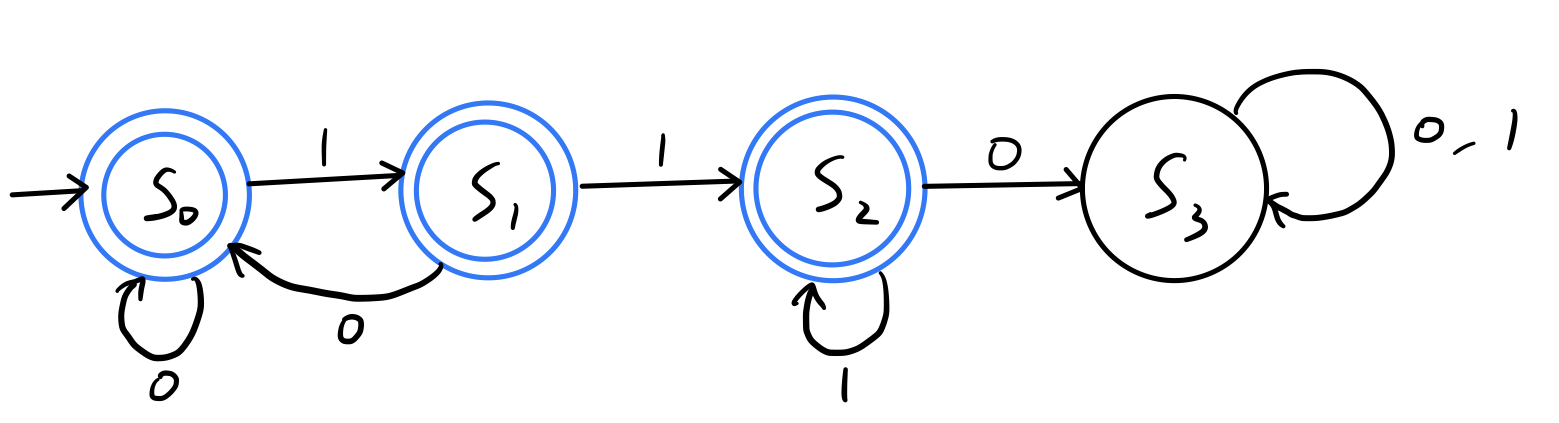
\includegraphics[width=10cm]{image/1.6.1.png}
        \caption{1.6.1}
        \label{fig:1_6f}
    \end{figure}

    蓝色双圆圈的状态表示接受状态. 下均同此表示.
\end{proof}

\problem{i.} $\{\omega \mid \omega \text{的奇数位置均为}1\}$

\begin{proof}
    \begin{figure}[!htbp]
        \centering
        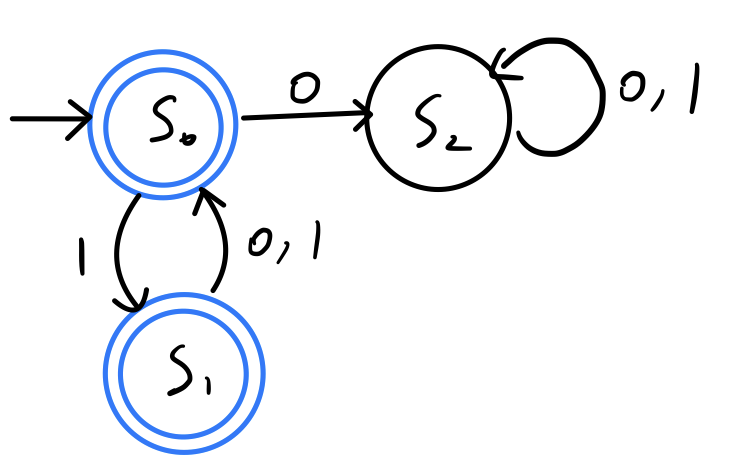
\includegraphics[width=6cm]{image/1.6.2.png}
        \caption{1.6.2}
        \label{fig:1_6i}
    \end{figure}

    如上图所示.
\end{proof}

\problem{1.14} 

\problem{a.} 证明: 若M是一台识别语言$B$的DFA, 交换M的接受状态与非接受状态得到一台新的DFA, 则这台新DFA识别$B$的补集. 因而, 正则语言类在补运算下封闭.

\begin{proof}
    M这台DFA在接收一串字符后, 按照定义, 会停止在一个确定的位置. 一个字符串$\omega$要么会让M停止在接受状态, 这时$\omega \in B$, 要么会让M停止在非接受状态, 这时$\omega \notin B$. 如果让接受状态与非接受状态交换, 记$B'$为新的DFA (记作M') 所识别的语言, 那么原本被接受的字符串$\omega$就会不被新的DFA接受, 于是$\omega \notin B'$, 原本不被接受的字符串现在被$B'$接受, 因而$\omega \in B'$. 于是根据定义, $\forall\,\omega\in B (\omega \notin B') \land \forall\,\omega\notin B (\omega \in B')$, 所以$B'$是$B$的补集, 即这台新DFA识别B的补集, $B'$也是正则语言. 由于M的任意性, 我们可以得到正则语言类在补运算下封闭的结论.
\end{proof}
    
\problem{b.} 举例说明: 若M是一台识别语言$C$的NFA, 交换M的接受状态与非接受状态, 得到一台新NFA, 这台NFA不一定识别$C$的补集. NFA识别的语言类在补运算下封闭吗? 并解释回答.

\begin{proof}
    新NFA不识别$C$的补集的例子如图\ref{fig:1_14b}:
    
    \begin{figure}[!htbp]
        \centering
        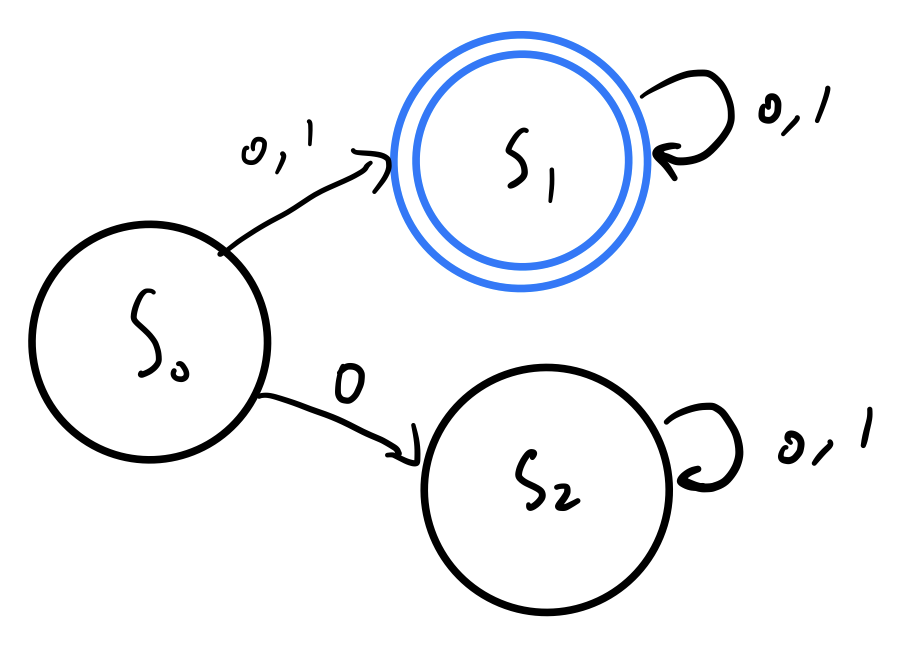
\includegraphics[width=5cm]{image/1.14.png}
        \caption{1.14}
        \label{fig:1_14b}
    \end{figure}
    
    考虑字符串 $0$, 无论是该NFA还是其接受状态与非接受状态交换后得到的新NFA, $0$ 均为被接受的输入, 因此这台特殊的NFA不识别 $C$ 的补集.
    
    但是, NFA识别的语言类在补运算下封闭. 题目只是指出, NFA的接受状态与非接受状态对换后, 新NFA的识别语言并不是原识别语言 $C$ 的补集, 并不是说原识别语言 $C$ 的补集就不是正则语言. 我们知道, 每一台NFA都等价于某一台DFA, 这样我们可以找到一台DFA, 并将之接受状态与非接受状态交换, 得到识别语言是 $C$ 的补集的一台状态机 M'; 再构造一个NFA, 使得NFA的状态图中, 所有状态和边都和M'相同. 这样, 这台NFA便满足题目要求, NFA识别的语言类在补运算下封闭.
\end{proof}

\problem{1.31} 对语言A和语言B, 设A和B的完全间隔交叉 (perfect shuffle) 为:
\[
    \{ \omega \mid \omega = a_1b_1 \,\cdots\, a_kb_k,\text{ 其中 } a_1\,\cdots\, a_k \in A \text{ 并且 } b_1\,\cdots\, b_k \in B, \text{ 任一 } a_i,b_i\in\Sigma \}
\]
证明: 正则语言类在完全间隔交叉下封闭.

\begin{proof}
    第一步是依据某个已有DFA构造一个新DFA, 只读取奇/偶数位的输入, 并且接收相同的字符串 (对奇/偶数位). 我们只讨论 "只读取奇数位输入的新DFA构造", 因为偶数位的原理相同.
    
    对于一个名为$M$的DFA, 分别用 $S_0, S_1,\,\dots\,,S_n$ 来表示它的$n+1$个不同状态. 我们现构造一个新的DFA, 名为$M'$, 它拥有$2n+2$个不同的状态, 分别是 $S_{\text{a}0}, S_{\text{a}1},\,\dots\,,S_{\text{a}n},S_{\text{b}0}, S_{\text{b}1},\,\dots\,,S_{\text{b}n}$. $M'$的状态转移依照如下定义给定:

    \begin{enumerate}
        \item 如果$M$中有$S_i\times \alpha \xrightarrow{\delta} S_j,\ S_i, S_j\in Q,\ \alpha\in\Sigma$, 那么在$M'$中构造一条状态转移: $S_{\text{a}i}\times \alpha \xrightarrow{\delta} S_{\text{b}j},\ S_{\text{a}i}, S_{\text{b}j}\in Q',\ \alpha\in\Sigma$, 其中$Q, Q'$分别为$M,M'$的状态集合. 这个定义负责读取奇数位的输入.
        \item $\forall i\in \{0,1,\,\dots\,,n\}\,,\ \forall \alpha\in\Sigma$, 构造转移: $S_{\text{b}i}\times \alpha \xrightarrow{\delta} S_{\text{a}i},\ S_{\text{b}i}, S_{\text{a}i}\in Q'$. 这个定义负责忽略偶数位的输入.
    \end{enumerate}

    在此之后, 我们还需要定义新的接收状态. 如果$M$的接受状态集合为$S_{r_0},\, S_{r_1},\,\dots\,,\,S_{r_n}$, 那么$M'$的接受状态集合就应该被定义为$S_{\text{a}r_0},\, S_{\text{a}r_1},\,\dots\,,\,S_{\text{a}r_n}$. 根据推理可知, 状态转移图是一个二部图, 因此, a表示的是定义了原本下标中数字对应的新的两个状态中, 表明已读取数字为偶数的一个状态. 这样$M'$只会接受长度为偶数的字符串.
    
    只读取偶数位置输入的构造同理, 要求也是必须输入字符串偶数长才能接受.

    既然这样可以构造出两种DFA, 那么这两种构造后的接受语言也都是正则语言, 因此对正则语言类, 此种构造是封闭的.
    
    第二步是证明引理: 正则语言类在交下是封闭的. 首先定义两个语言的交为: $A\cap B = \{ x\mid x\in A \text{ 且 } x\in B \}$. 使用和证明并运算封闭的方法类似, 只不过定义 $F = \{ (r_1,r_2)\mid r_1\in F_1 \text{ 且 } r_2\in F_2 \}$, 之后引理显然可证.
    
    第三步是把$A$和$B$对应的状态机分别取奇数位有效和偶数位有效的变换, 然后交在一起. 这两步都封闭的话, 两步运算的符合还是封闭的, 于是得到的语言仍然是正则语言. 根据定义, 我们能够给出得到的语言的定义: 奇数位相连是$A$对应的接受语言中的字符串, 偶数位相连是$B$对应的接受语言中的字符串, 并且此字符串必须是偶数为长度. 这与题目对完全间隔交叉的定义如出一辙, 即$\{\omega \mid \omega = a_1b_1 \,\cdots\, a_kb_k,\text{ 其中 } a_1\,\cdots\, a_k \in A \text{ 并且 } b_1\,\cdots\, b_k \in B, \text{ 任一 } a_i,b_i\in\Sigma\}$. 因此, 正则语言类在完全间隔交叉下封闭, 题目得证.
    
\end{proof}

\problem{1.35} 设 $A/B = \{ \omega\mid\text{ 对于某 }x\in B, \omega x\in A \}$. 证明如果 $A$ 是正则的, $B$ 是任意语言, 那么 $A/B$ 是正则的.

\begin{proof}
    记正则语言 $A$ 对应的某一个DFA为 $M = \{ Q,\,\Sigma,\,\delta:Q\times\Sigma\rightarrow Q,\,q_0\in Q,\,F\subseteq Q \}$. 记函数 $\vartheta: Q\times\Sigma \rightarrow 2^Q$ 满足:
    \[
        \forall q \in Q,\ \forall \sigma \in \Sigma,\ \vartheta(q, \sigma) = \{q'\mid \delta(q', \sigma) = q\}
    \]
    即$\vartheta$是一个在同一字母下将所有转移反向的函数. 然后扩充定义这个函数对字符串的操作, 即从前向后依次对字符串中的每一个字母进行映射操作; 对集合的操作, 即分别对集合中的每一个字母/字符串进行映射操作. 总之, 定义此函数使我们可以回溯DFA的转移步骤.

    定义对语言的反转为 $L^R = \{\omega^R \mid \forall\omega\in L\}$. 集合 $C := \vartheta(F, B^R)$, 这表示从该DFA的每一个接受状态开始, 对语言$B$的所有字符串的反转进行回溯, 得到的状态的集合. 满足 $\forall q\in C, \exists \omega\in B, \exists q'\in F\,\,(\delta(q,\omega) = q')$. 容易证明, 这个定义等价于:
    \[
        C = \{ q\mid q = \delta(q_0, A/B) \}
    \]
    所以我们只需要把由$A$定义出的DFA中, 接受状态集$F$替换成$C$, 就可以得到一个对应接收语言为$A/B$的DFA, 所以$A/B$也是正则的. 
\end{proof}




\textbf{第1.2次作业: 1.16 (b) 1.21 (b) 1.28 (a)}

\problem{1.16} 使用定理1.19给出的构造, 把下图的两台非确定型有穷自动机转换成等价的确定型有穷自动机.

\problem{b.} 如图\ref{fig:1_16b}

\begin{figure}[!htbp]
    \centering
    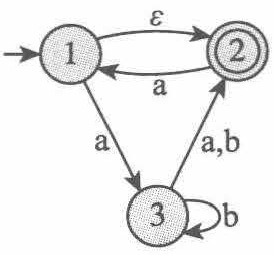
\includegraphics[height=3cm]{image/1.16 b.png}
    \caption{1.16 (b) 题目图片}
    \label{fig:1_16b}
\end{figure}

\begin{proof}
    如图\ref{fig:1_16}

    \begin{figure}[!htbp]
        \centering
        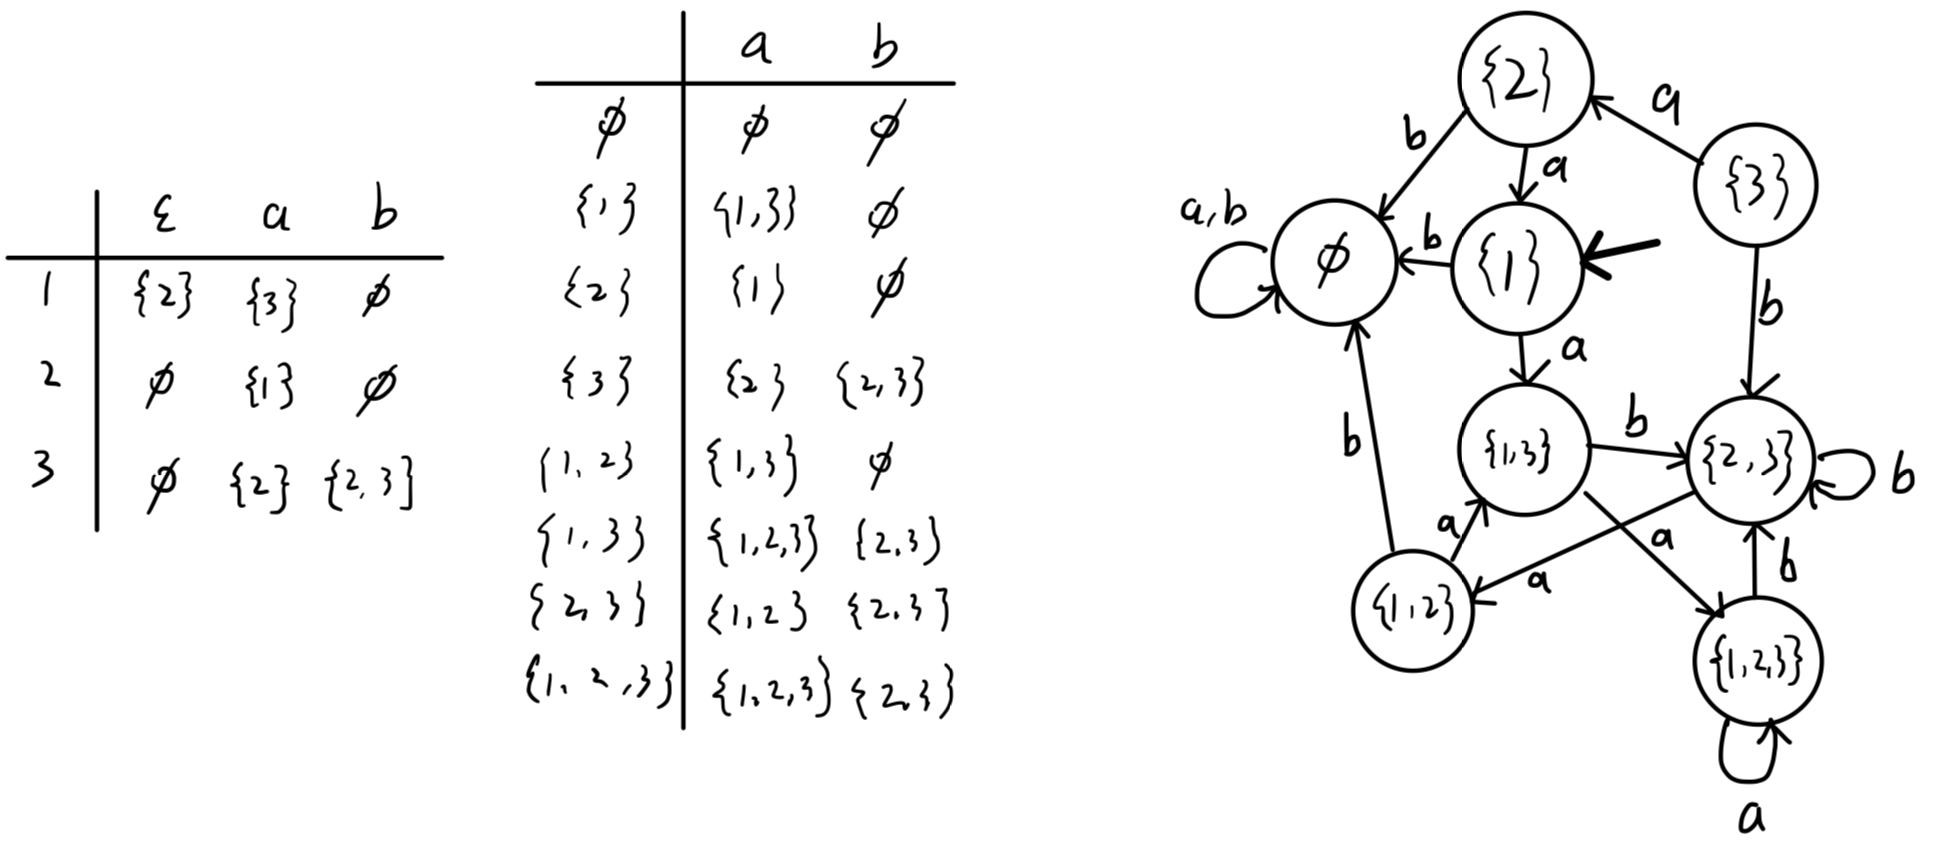
\includegraphics[height=5cm]{image/1.16.png}
        \caption{1.16 (b)}
        \label{fig:1_16}
    \end{figure}
\end{proof}

\problem{1.21} 使用引理1.32中描述的过程, 把下述有穷自动机转换成正则表达式.

\problem{b.} 如图\ref{fig:1_21b}

\begin{figure}[!htbp]
    \centering
    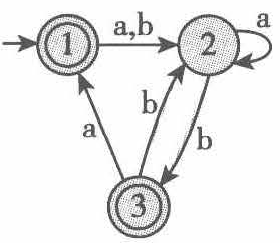
\includegraphics[height=3cm]{image/1.21 b.png}
    \caption{1.21 (b) 题目图片}
    \label{fig:1_21b}
\end{figure}

\begin{proof}
    如图\ref{fig:1_21}

    \begin{figure}[!htbp]
        \centering
        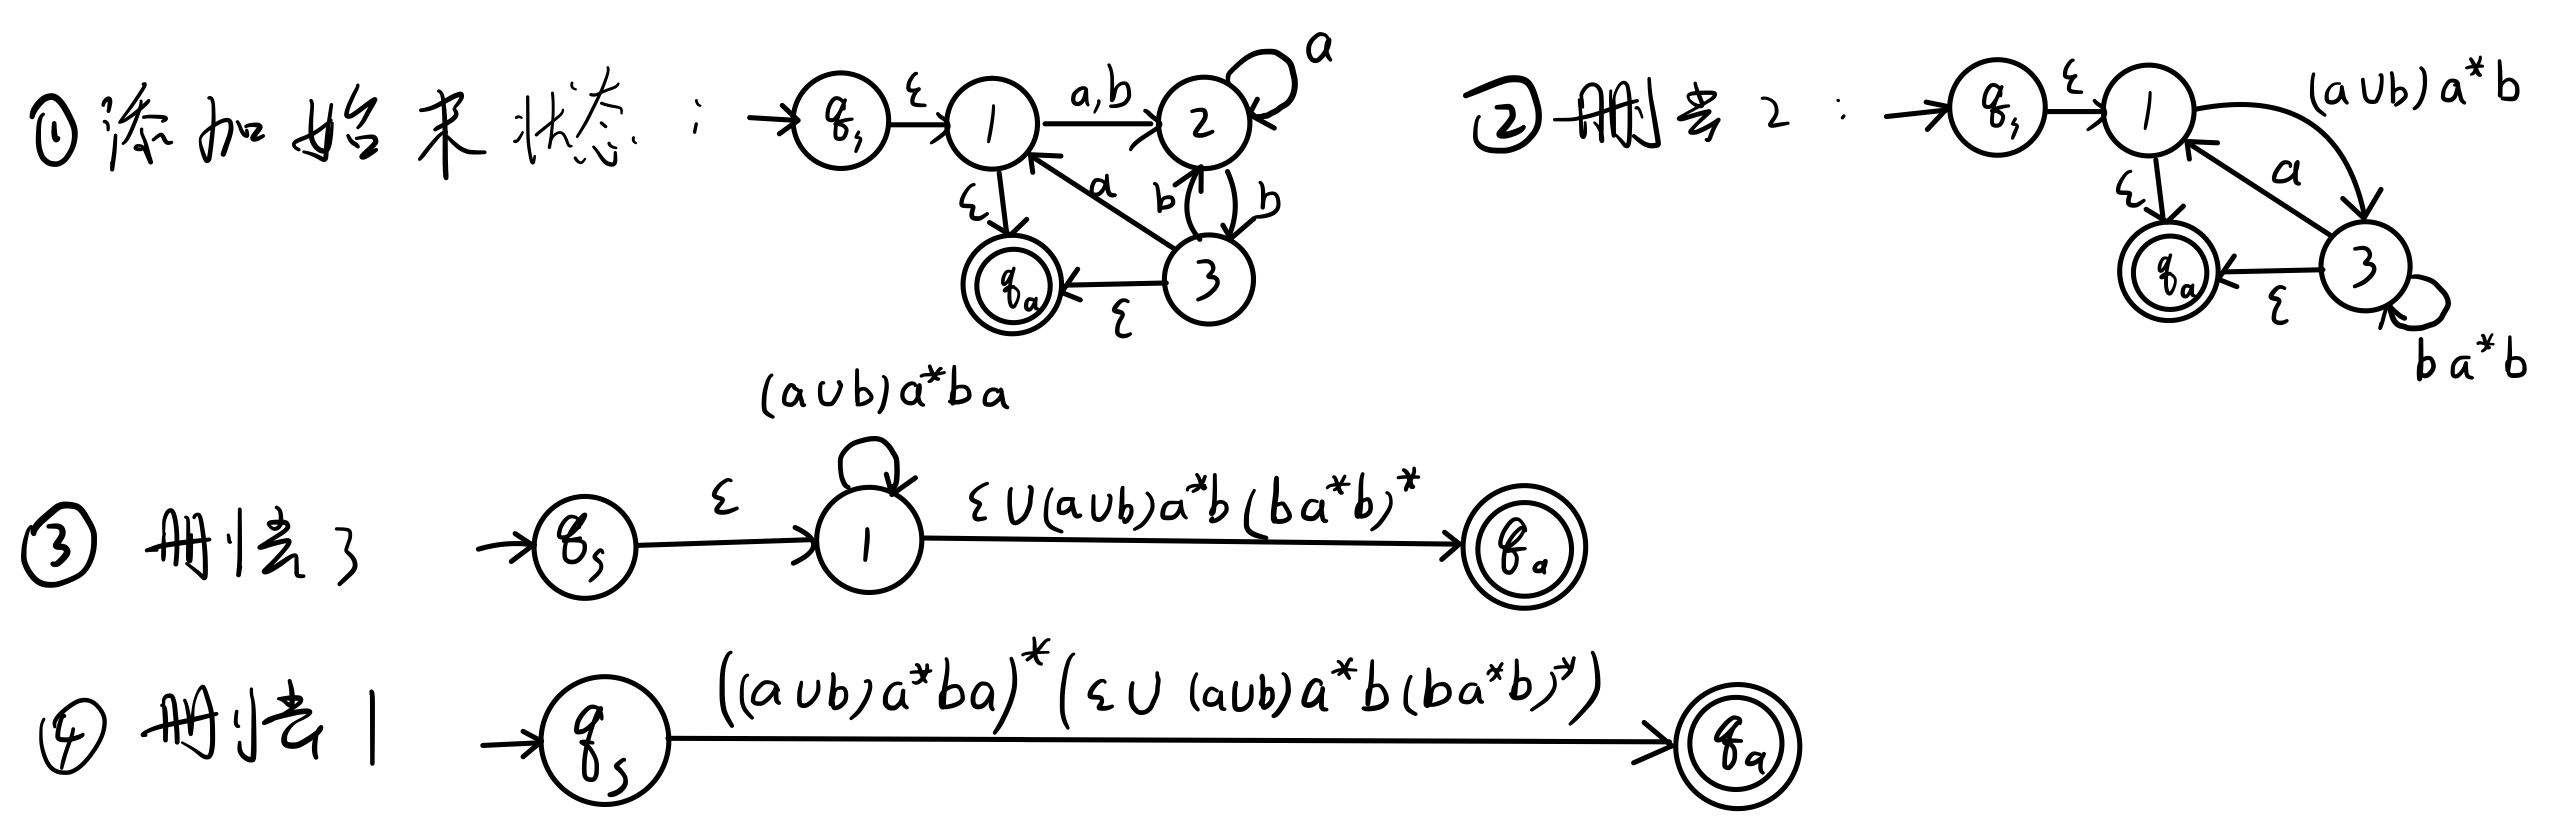
\includegraphics[height=5cm]{image/1.21.png}
        \caption{1.21 (b)}
        \label{fig:1_21}
    \end{figure}
\end{proof}


\problem{1.28} 使用定理1.28给出的过程将下述正则表达式转换成NFA. 在所有问题中 $\Sigma = \{ a,b \}$.

\problem{b} $a^+ \cup (ab)^+$

\begin{proof}
    如图\ref{fig:1_28}

    \begin{figure}[!htbp]
        \centering
        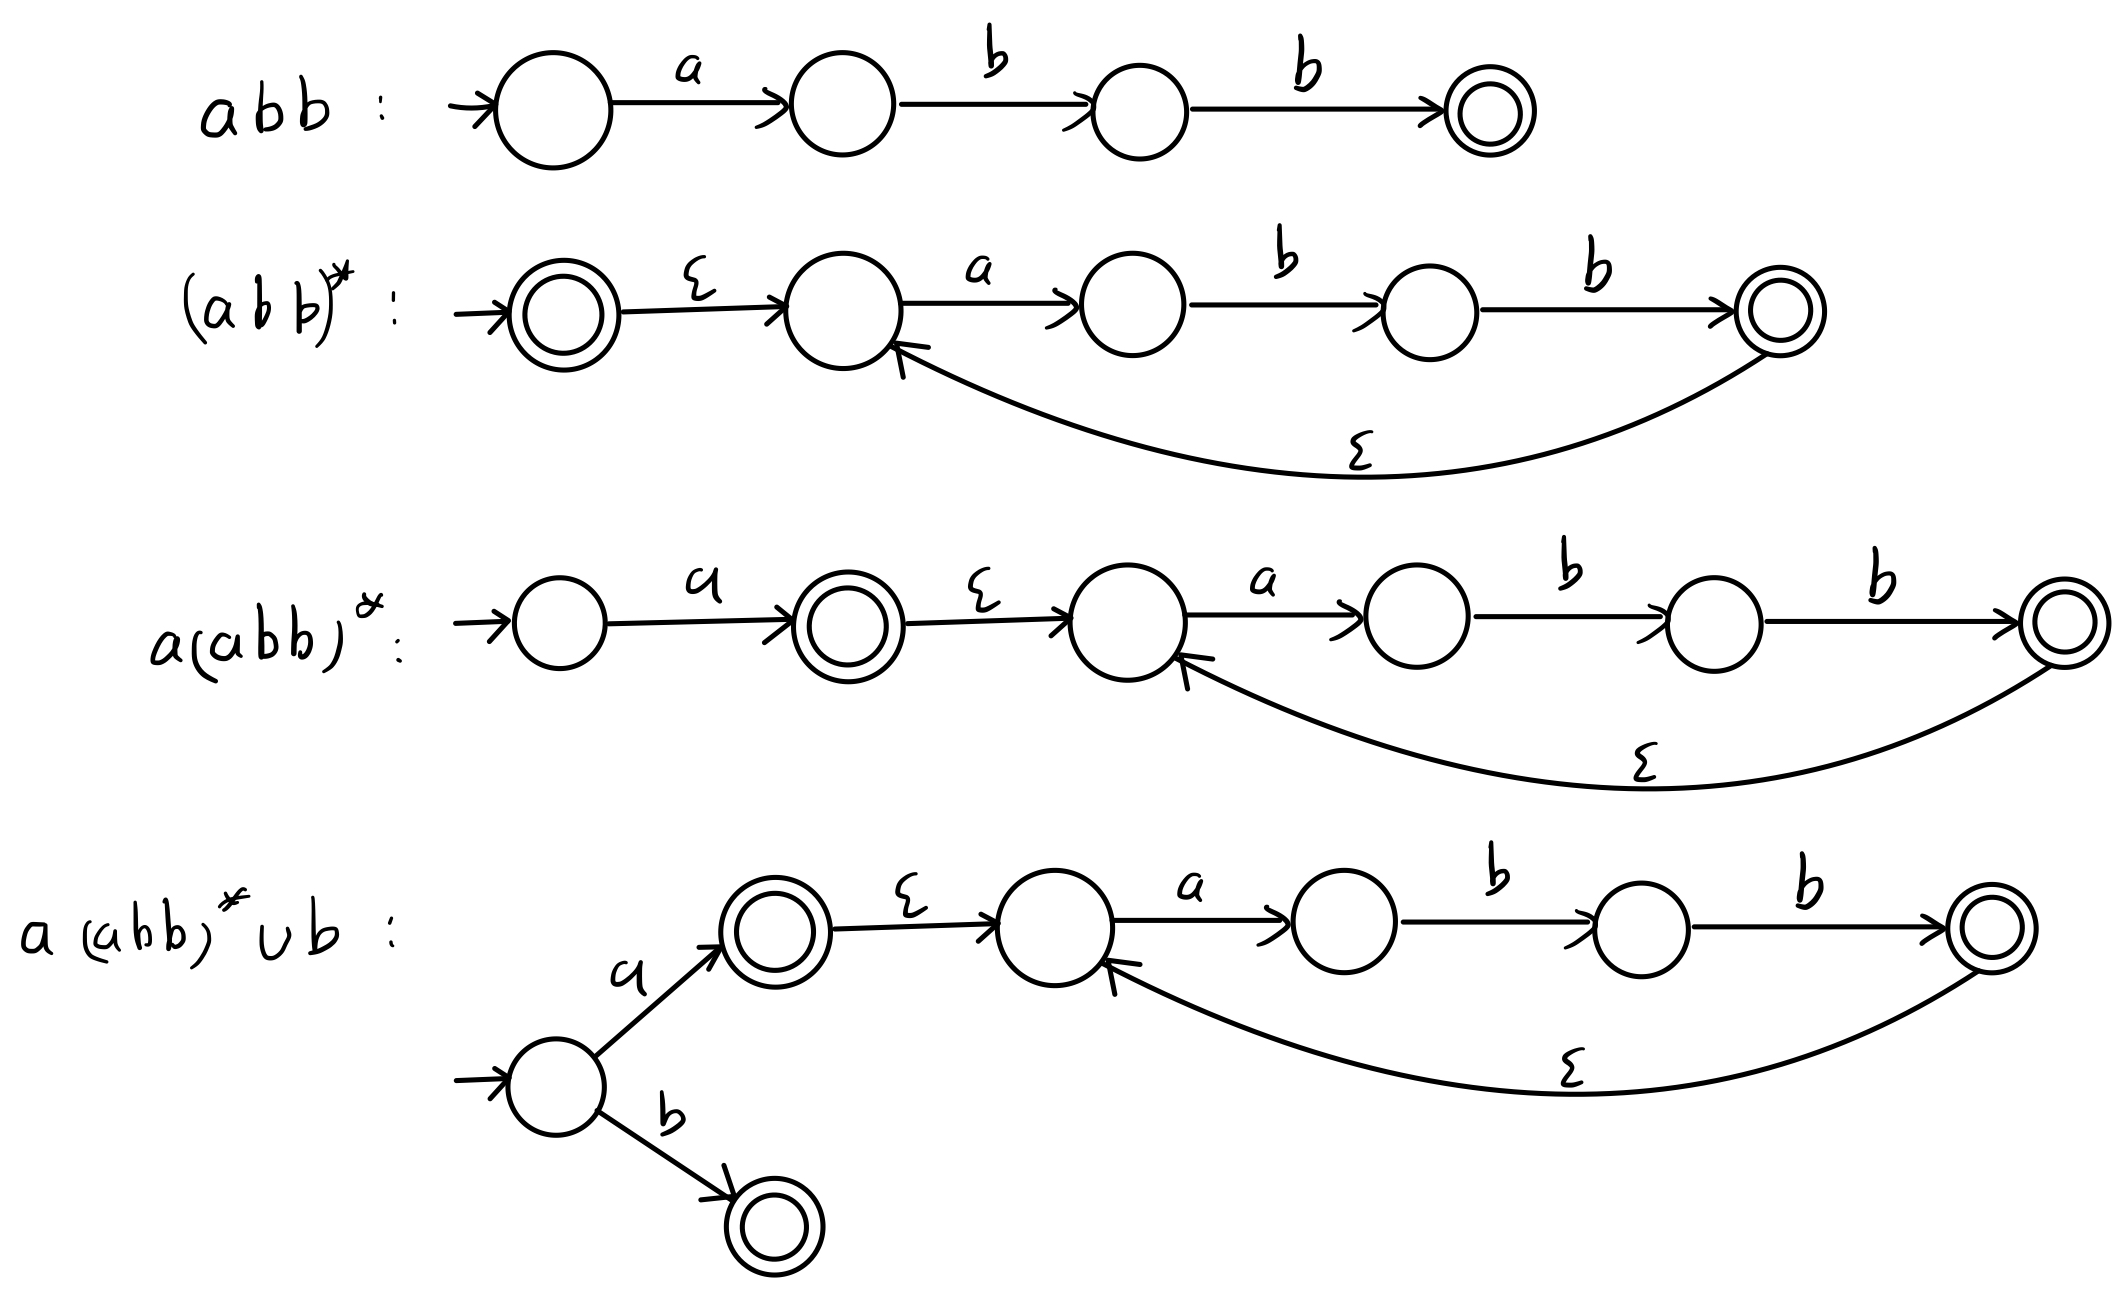
\includegraphics[height=7cm]{image/1.28.png}
        \caption{1.28 (b)}
        \label{fig:1_28}
    \end{figure}
\end{proof}






\textbf{第1.3次作业: 1.47, 1.48, 补充题3个, 其中2个选做}

\problem{1.47} 设$x$和$y$是两个字符串, $L$是一个语言. 如果存在字符串$z$, 使得$xz$和$yz$中恰好有一个是$L$的成员, 则称$x$和$y$是用$L$可区分的; 否则, 对每一个字符串$z$, $xz$和$yz$要么都是、要么都不是$L$的成员, 则称$x$和$y$是用$L$不可区分的. 如果$x$和$y$是用$L$不可区分的, 记作$x\equiv_L y$. 证明$\equiv_L$是一个等价关系. 

\begin{proof}
    等价关系的性质为: 对称性, 自反性和传递性, 下分别证明$\equiv_L$拥有这三个性质.

    对称性: 如果$x\equiv_L y$, 那么$x$和$y$是用$L$不可区分的, 这样对每一个字符串$z$, $xz$和$yz$要么都是、要么都不是$L$的成员. 这件事显然可以反过来, 于是$y$和$x$是用$L$不可区分的, 因此$y\equiv_L x$显然成立, 对称性成立.

    自反性: 显然, 对每一个字符串$z$, $xz$和$xz$作为完全相同的字符串, 要么都是、要么都不是$L$的成员. 因此$x\equiv_L x$, 自反性成立.

    传递性: 如果$x\equiv_L y$且$y\equiv_L w$, 那么对每一个字符串$z$, 
    $[(xz\in L \land yz\in L) \lor (xz\notin L \land yz\notin L)] \land [(yz\in L \land wz\in L) \lor (yz\notin L \land wz\notin L)]$. 经过逻辑化简, 我们可以得到$(xz\in L \land yz\in L \land wz\in L) \lor (xz\notin L \land yz\notin L \land wz\notin L)$, 这可以推出
    $(xz\in L \land wz\in L) \lor (xz\notin L \land wz\notin L)$. 这就是说, 对每一个字符串$z$, $xz$和$wz$要么都是、要么都不是$L$的成员, 所以$x\equiv_L w$, 传递性成立.
\end{proof}

\problem{1.48} Myhill-Nerode定理. 参见问题1.47, 设$L$是一个语言, $X$是一个字符串集合. 如果$X$中的任意两个不同的字符串都是用$L$可区分的, 则称$X$是用$L$两两可区分的. 定义$L$的指数为用$L$两两可区分的集合中的元素个数的最大值. $L$的指数可能是有穷的或无穷的. 

\problem{a.} 证明: 如果$L$被一台有$k$个状态的DFA识别, 则$L$的指数不超过$k$.

\begin{proof}
    那么$L$为一个正则语言. 记这台DFA为$M = (Q, \Sigma, \delta, q_0, F)$. 我们考虑一个映射$f$, 表示一个字符串被该DFA执行得到的结果状态, 有归纳定义如下:
    $f(\varepsilon) = q_0$;
    $\forall \omega\in\Sigma^*, \forall a\in\Sigma, f(\omega a) = \delta(f(\omega), a)$.

    这时我们定义另一个等价关系 (易证) $\forall x,y \in \Sigma^* , x\simeq y \Longleftrightarrow f(x) = f(y)$. 这样看来, $f$给出了一个蕴含了等价关系$\equiv_L$的等价关系, 因为$x\simeq y \rightarrow x\equiv_L y$. 这是因为, 后者的定义其实是$\forall z\in \Sigma^*, (f(xz)\in L\land f(yz)\in L) \lor (f(xz)\notin L\land f(yz)\notin L)$, 而$f(x) = f(y) \rightarrow f(xz) = f(yz) \rightarrow (f(xz)\in L\land f(yz)\in L) \lor (f(xz)\notin L\land f(yz)\notin L)$. 考虑到$L$在$\simeq$下的等价类取决于字符串运算后终点的位置, 也就是停止的状态, 而这种状态最多有$k$个, 所以$L$的指数 (也就是在$\equiv_L$下的等价类个数) 不可能超过$k$.
\end{proof}

\problem{b.} 证明: 如果$L$的指数是一个有穷数$k$, 则它被一台有$k$个状态的DFA识别.

\begin{proof}
    $L$的指数是一个有穷数$k$, 意味着任意字符串$z\in\Sigma^*$, 一共有至多$k$个$\equiv_L$下的等价类. 下面给出一种DFA的构造, 使得其接收语言$L$. 其中用到定义: $[x]_L$指$x$在$\equiv_L$下所在的等价类.

    定义DFA: $M = (Q, \Sigma, \delta, q_0, F)$, 满足:
    \begin{itemize}
        \item $Q = \{ [x]_L \mid x\in\Sigma^*\}$
        \item $\delta([x]_L, a) = [xa]_L$
        \item $q_0 = [\varepsilon]_L$
        \item $F = \{ [x]_L \mid x\in L \}$
    \end{itemize}

    为了证明$M$的接受语言就是$L$, 我们需要证明两件事: 一是$L$中的所有字符串都能够被$M$接受, 二是不在$L$中的所有字符串都不能够被$M$接受.

    \begin{enumerate}
        \item $\forall y\in L$, 将$y$放入自动机, 显然, 我们进入的状态就是$[y]_L\,,\ y\in L$ (可以由递归的定义接受字符串, 证明这件事), 而这正是一个被接受的状态.
        \item $\forall y\notin L$, 将$y$放入自动机, 进入的状态就是$[y]_L\,,\ y\notin L$. 另$\forall x\in L$, 存在一个空串$\varepsilon$使得$x\varepsilon \in L\ \land\ y\varepsilon \notin L$, 因此$x$与$y$是用$L$不可区分的, 因此$y \notin \{ [x]_L \mid x\in L \} = F$, 即非语言$L$中的字符串都是不被$M$接受的.
    \end{enumerate}
    
    根据以上两面的论述, 我们得知$M$的接受语言确是$L$; 而$M$的状态数就是$L$的指数$k$, 证毕.
\end{proof}

\problem{c.} 由此得到: $L$是正则的当且仅当它有有穷的指数. 而且, 它的指数是识别它的最小DFA的大小.

\begin{proof}
    根据a得出, $L$是正则的 (被一台DFA识别), 仅当它有有穷的指数, 且它的指数不超过DFA的状态数.

    根据b得出, $L$是正则的, 当它有有穷的指数, 且它的指数是一台识别它的DFA的状态数.

    a和b一同给出: $L$是正则的当且仅当它有有穷的指数. 

    b给出了a中$L$的指数可以是DFA状态数的构造, 因此我们可以得出, $L$的指数是识别它的最小DFA的大小.
\end{proof}


\problem{补充题1} 证明$\{ 0^m1^n \mid m > n \}$不是正则语言.

\begin{proof}
    泵引理: 对于任意的 (无穷) 正则语言$A$, 存在正整数$p$ (称为泵长度), 使得对于任意$\omega \in A$,如果$|\omega| ≥ p$, 则$\omega$可被分成$3$段,即$\omega = xyz$, 且$|y|\geq 1$, $|xy|\leq p$, 且对于任意$r\geq 0,\, xy^rz\in A$.

    仔细观察泵引理的证明过程, 发现是使用$i\in\{0,\,1,\,2,\,\dots\,,\,p\}$这前$p$个状态证明的, 只要换成$i\in\{S-p-1,\,S-p,\,S-p+1,\,\dots\,,\,S-1\}$ ($S$表示状态数) 这后$p$个 (除去最后一个状态), 可以得到与最后的状态有关的 "泵引理", 即将条件中的$|xy|\leq p$改为$|yz|\leq p$.

    使用这个新的 "泵引理", 并假设这个语言是正则的, 那么存在$p$使得泵引理的条件满足. 记此语言为$L$, 我们可以取$\omega\in L$满足$n>p+3$, 这样$\omega = xyz$中的$x$一定全部由$1$组成. 取$r = m+1$, 显然$xy^rz = 0^m1^{n+m|y|}$, 其中$n+m|y|>m$, 与$xy^rz\in L$矛盾! 故$L$不是正则语言.
\end{proof}

\problem{(选做) 补充题2} 证明$\{ 0^m1^n \mid m \neq n \}$不是正则语言. (懒得想了)

\problem{(选做) 补充题3}:证明$\{ 1^n \mid n\text{是素数} \}$不是正则语言.

\begin{proof}
    考虑泵引理, 假设题中语言 (记为$L$) 是正则语言, 则$\exists p\in\Z^+$使得$\omega\in L \,\land\, |\omega|\geq p$, $\omega = xyz\ , |y| \geq 1\,, |xy| \leq p\,, \forall r\geq 0\, (xy^rz\in L)$.
    
    寻找反例: $r = |\omega|-|y|$, 那么:
    \[
        |xy^rz| = |x| + r|y| + |z| = |y|(|\omega|-|y|) + |\omega|-|y| = (|y| + 1)(|\omega|-|y|)
    \]
    显然这样的字符串长度不为质数, 导出矛盾! 因此不能满足泵引理, $L$不是正则语言.
\end{proof}




















%\bibliographystyle{amsalpha}
%\bibliography{all-bibliography}
%\addcontentsline{toc}{section}{References}


\end{document}